\section{Versuch 3: $\gamma$-Koinzidenzspektroskopie}
\subsection{Aufgaben}
\begin{enumerate}
    \item Messung des $\gamma$-Spektrums von \ce{^22Na}, \ce{^137Cs} und \ce{^60Co} mit beiden Detektoren (NaI-Detektor und Ge-Detektor). Energiekalibration mit Hilfe der Photopeaks.
    \item Koinzidenzmessung mit \ce{^22Na} und \ce{^60Co} Quellen.
    \begin{enumerate}
        \item $\Delta T$ Kalibration mit der \ce{^22Na} Quelle.
        \item Analyse der Koinzidenzen. Zwischen welchen Photonen gibt es eine signifikante korrelation? Mit welchem Termschema kann man diese erklären? Gibt es weitere Koinzidenzen?
    \end{enumerate}
    \item Analyse der Abhängigkeit der Energieauflösung des Ge-Detektors und des NaI-Detektors von der Energie. Wie lässt sich der Unterschied erklären?
\end{enumerate}

\newcommand{\weirdertext}{1.332MeV \\[-.5\baselineskip] % Adjust vertical space as needed
    \phantom{1.332MeV} or \\[-.5\baselineskip] % Adjust vertical space as needed
    1.173MeV}

\begin{figure}[b]
    \centering
    \begin{subfigure}{0.4\textwidth}
        \centering
        \begin{tikzpicture}[>=stealth,thick]
            \draw(0,4) -- (2,4) node[midway,above] {\ce{^{60}Co}};
            \draw(2,3) -- (4,3);
            \draw(2,2) -- (3,2);
            \draw[dashed](3.4,2) -- (3,2);
            \draw[dashed](3.6,2) -- (4,2);
            \node at (5,3) {1.332MeV};
            \node at (5,2) {1.173MeV};
            \draw(2,0) -- (4,0) node[midway,below] {\ce{^{60}Ni}};
            \draw[->] (1,4) -- (2,3) node[midway, right, xshift=2.5, yshift=2.5]{$\beta_2$};
            \draw[->] (1,4) -- (2,2) node[midway, left]{$\beta_1$};
            \draw[->] (2.5,2) -- (2.5,0) node[midway, right]{$\gamma_1$};
            \draw[->] (3.5,3) -- (3.5, 0) node[midway, right]{$\gamma_2$};
        \end{tikzpicture}
        \caption{Independant Decay}
        \label{fig:termschema:independant}
    \end{subfigure}%
    \begin{subfigure}{0.4\textwidth}
        \centering
        \begin{tikzpicture}[>=stealth,thick]
            \draw(0,4) -- (2,4) node[midway,above] {\ce{^{60}Co}};
            \draw(2,3) -- (4,3);
            \node[anchor=west, align=left] at (4,3) {2.505MeV};
            \node[anchor=west, align=left] at (4,1.5) {\weirdertext};
            \draw(2,1.5) -- (4,1.5);
            \draw(2,0) -- (4,0) node[midway,below] {\ce{^{60}Ni}};
            \draw[->] (1,4) -- (2,3) node[midway, right, xshift=2.5, yshift=2.5]{$\beta$};
            \draw[->] (3,3) -- (3,1.5) node[midway, right]{$\gamma_a$};
            \draw[->] (3,1.5) -- (3,0) node[midway, right]{$\gamma_b$};
        \end{tikzpicture}
        \caption{Cascade}
        \label{fig:termscheme:cascade}
    \end{subfigure}
    \caption{Mögliche Termschemata für den Zweiquantenzerfall.}
    \label{fig:termscheme}

\end{figure}



%\SI{1.332}{\MeV} \\ or\\ \SI{1.173}{\MeV}

\subsection{Einführung}
Ein Kern emittiert $\gamma$-Quanten, wenn er sich nach vorausgegangenem $\alpha$ oder $\beta$-Zerfall oder infolge einer Kernreaktion in einem angergeten Zustand befindet. Der Übergang in den Grundzustand kann dabei in einem Schritt und/oder stufenweise erfolgen. In diesem Fall spricht man von $\gamma$-Kaskaden. Bei hoch angeregten Kernen sind i.a. mehrere Wege zum Grundzustand möglich. Die relative Häufigkeit eines bestimmten Weges hängt von den Quantenzahlen der Spins der beteiligten Zustände und deren Parität ab und wird durch das sog. Verzweigungsverhältnis ausgedrückt. Ziel der $\gamma$-Spektroskopie ist es, die Energie und die Quantenzahlen der Zustände zu bestimmen.

In diesem Versuch wird eine Methode vorgestellt, die ein erster Schritt zur Festlegung des Termschemas von Kernen ist, die Koinzidenzspektroskopie. Sie ist auch ein wesentlicher Bestandteil von weiterführenden Experimenten zur Bestimmung der Quantenzahlen, wie z.B. der Messung der Winkelkorrelation.

Die Koinzidenzmethode, ursprünglich von W. Bothe und H. Geiger entwickelt, ist eine Methode um zwischen Hintergrund und relevanten Ereignissen zu unterscheiden. Dies ist möglich sofern die interessanten Ereignisse über mehrere Kanäle gleichzeitig registriert werden, während die hintergrund Ereignisse immer nur in einzelnen Kanälen auftreten.
Die hintergrund Prozesse können meist als unabhängige Poisson verteilte Ereignisse mit einer Rate $\nu_i$ in Detektor $i$ modelliert werden. Diese hintergrund Prozesse erzeugen zufällige Koinzidenz Ereignisse, die wiederum Poisson verteilt mit einer Rate von $\nu_1\cdot\nu_2\cdot\Delta T$ sind. $\Delta T$ bezeichnet hierbei die Zeitspanne in denen ein Koinzidenz Ereignis auftreten muss um als solches registriert zu werden.

\subsection{Prinzip der Messung}
Der Versuchsaufbau besteht aus zwei $\gamma$-Detektoren (NaI-Szintillator und HPGe-Halbleiterzähler), deren Energiesignale von einem RedPitaya ausgelesen werden. Der RedPitaya fungiert als Oszilloskop und nimmt beide Kanäle gleichzeitig auf. Das Oszilloskop wird von einem Kanal getriggert. Findet sich in dem anderen Kanal ebenfalls ein Puls spricht man von einem Koinzidenzereignis.
%Die Oszilloskop Daten werden an mimoCoRB (multiple-in, multiple-out Configurable RingBuffer) übertragen und dort analysiert.
Im ersten Schritt werden mit bekannten Eichquellen die Energieskalen kalibriert. Mithilfe der bekannten Koinzidenz der \ce{^22Na} Quelle wird die Zeitdifferenz der Pulse kalibriert.

\ce{^60Co} ist ein $\beta^{-}$-Strahler mit zwei $\gamma$-Übergängen (1,173 MeV und 1,332 MeV), wie man aus den Einzelspektren entnimmt. Für das Termschema gibt es damit prinzipiell die zwei in Fig. \ref{fig:termscheme} dargestellten Möglichkeiten. In Fall a) werden die angeregten Zustände durch zwei unabhängige $\beta$-Übergänge besetzt. Deshalb werden auch die $\gamma$-Quanten zeitlich unabhängig voneinander emittiert. Anders der Fall b). Dort gibt es nur einen $\beta$-Zerfall zum höchsten angeregten Zustand, und die folgenden $\gamma$-Quanten bilden den einfachsten Fall einer Kaskade. Wenn der Zwischenzustand hinreichend kurzlebig ist, bei \ce{^60Co} ist das mit $10^{-12}\mathrm{s}$ der Fall, treten die beiden Quanten praktisch gleichzeitig auf. Durch ein Koinzidenexperiment, bei dem die Gleichzeitigkeit der Zerfälle geprüft wird, kann man zwischen den beiden Möglichkeiten unterscheiden. Mithilfe eines Likelihood Ratio Tests kann die Signifikanz der Koinzidenzen bestimmt werden. Hierzu vergleicht man die Hypothese \emph{Es gibt keine Koinzidenzen} mit der Hypothese \emph{Es gibt Koinzidenzen}.


Die Anordnung des Experiments ist in Fig. \ref{fig:anordnung} skizziert. Das analoge Signal der Detektoren ist zunächst (vor-)verstärkt und dann von dem RedPitaya in ein digitales Signal umgewandelt. Der CIC Filter wird als Dezimationsfilter verwendet und erlaubt es die 125MegaSamples/s zu reduzieren. Wird das Oszilloskop getriggert, so werden die Daten von dem CPU an den mimoCoRB client übetragen. mimoCoRB erlaubt es diese Daten beliebig zu analysieren. Für den Versuch stehen zwei setups bereit. Das erste setup analysiert den Trigger Kanal bezüglich der Pulshöhe und erstellt daraus ein Spektrum. Das zweite setup untersucht beide Kanäle nach Ereignissen. Sofern in beiden Kanälen ein Ereignis gefunden wurde, werden sowohl die Pulshöhen als auch die Zeitdifferenz gespeichert. Zusätzlich können die Daten in beiden Moden live visualisiert werden.

\usetikzlibrary{snakes}

\begin{figure}[tb]
    \centering
    
    
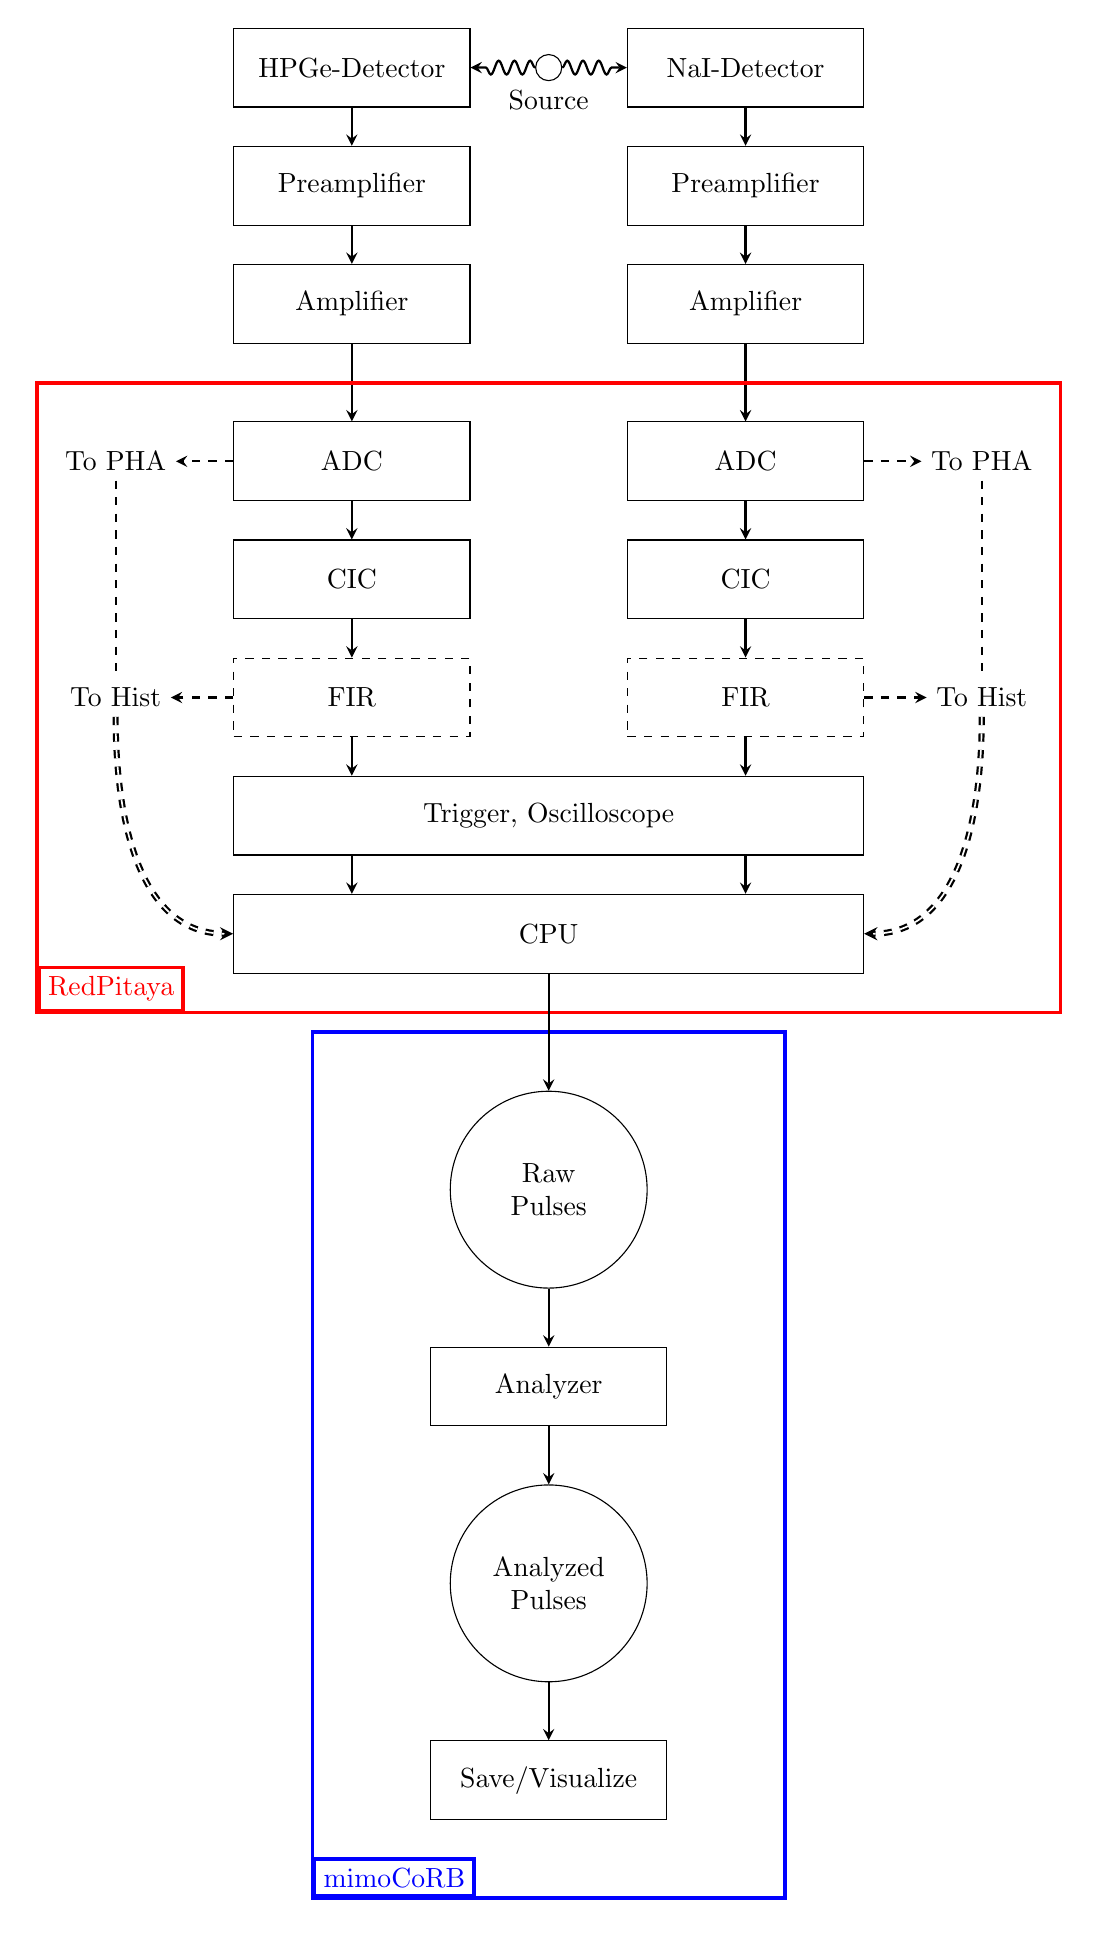
\begin{tikzpicture}[node distance=1.5cm]
\tikzstyle{Module} = [rectangle,  minimum width=3cm, minimum height=1cm,align=center, draw=black]
\tikzstyle{ModuleDummy} = [rectangle,  minimum width=3cm, minimum height=1cm,text centered, draw=none]
\tikzstyle{Trash} = [rectangle, minimum width=1cm, draw=none]
\tikzstyle{source} = [circle, text centered, minimum size=.2cm, draw=black, label=below:{Source}]
\tikzstyle{Both} = [rectangle, minimum width=8cm, minimum height=1cm,text centered, draw=black]

\tikzstyle{RB} = [circle, align=center, minimum size=2.5cm, draw=black]

\tikzstyle{arrow} = [thick,->,>=stealth]
\tikzstyle{line} = [thick]


\def\xsep{4cm}


\def\xtrash{1.5cm}


\node (source) [source] at (0,0) {};

\node[Module, right of =source, xshift=1cm] (Na) {NaI-Detector};
\node[Module, left of =source, xshift=-1cm] (Ge) {HPGe-Detector};


\draw[arrow,decorate, decoration={snake, segment length=2mm, post length=1.5mm}] (source) -- (Na);
\draw[arrow,decorate, decoration={snake, segment length=2mm, post length=1.5mm, mirror}] (source) -- (Ge);

\node[Module, below of =Na] (NPreAmp) {Preamplifier};
\node[Module, below of =Ge] (GPreAmp) {Preamplifier};
\draw[arrow] (Na) -- (NPreAmp);
\draw[arrow] (Ge) -- (GPreAmp);

\node[Module, below of =NPreAmp] (NAmp) {Amplifier};
\node[Module, below of =GPreAmp] (GAmp) {Amplifier};
\draw[arrow] (NPreAmp) -- (NAmp);
\draw[arrow] (GPreAmp) -- (GAmp);




\node[Module, below of =NAmp, yshift=-.5cm] (NADC) {ADC};
\node[Module, below of =GAmp, yshift=-.5cm] (GADC) {ADC};
\draw[arrow] (NAmp) -- (NADC);
\draw[arrow] (GAmp) -- (GADC);



\node[Module, below of =NADC] (NCIC) {CIC};
\node[Module, below of =GADC] (GCIC) {CIC};
\draw[arrow] (NADC) -- (NCIC);
\draw[arrow] (GADC) -- (GCIC);

\node[Module, below of =NCIC, dashed] (NFIR) {FIR};
\node[Module, below of =GCIC, dashed] (GFIR) {FIR};
\draw[arrow] (NCIC) -- (NFIR);
\draw[arrow] (GCIC) -- (GFIR);



\node[ModuleDummy, below of=NFIR] (NTrigOsc) {};
\node[ModuleDummy, below of=GFIR] (GTrigOsc) {};
\draw[arrow] (NFIR) -- (NTrigOsc);
\draw[arrow] (GFIR) -- (GTrigOsc);

\node[Both, below of =source, yshift=-8cm] (TrigOsc) {Trigger, Oscilloscope};
\node[Both, below of =TrigOsc] (CPU) {CPU};

\node[ModuleDummy, below of=NTrigOsc] (NCPU) {};
\node[ModuleDummy, below of=GTrigOsc] (GCPU) {};
\draw[arrow] (NTrigOsc) -- (NCPU);
\draw[arrow] (GTrigOsc) -- (GCPU);

% Trash
\node[Trash, right of=NADC, xshift=+\xtrash] (NPHA) {To PHA};
\node[Trash, left of=GADC, xshift=-\xtrash] (GPHA) {To PHA};
\draw[arrow, dashed] (NADC) -- (NPHA);
\draw[arrow, dashed] (GADC) -- (GPHA);

\node[Trash, right of=NFIR, xshift=+\xtrash] (NHist) {To Hist};
\node[Trash, left of=GFIR, xshift=-\xtrash] (GHist) {To Hist};
\draw[arrow, dashed] (NFIR) -- (NHist);
\draw[arrow, dashed] (GFIR) -- (GHist);

\node[Trash, right of=NCPU, xshift=+\xtrash] (NTrash) {};
\node[Trash, left of=GCPU, xshift=-\xtrash] (GTrash) {};
\draw[line, dashed] (NPHA) -- (NHist);
\draw[line, dashed] (GPHA) -- (GHist);
\draw[arrow, double, dashed] (NHist) to[out=-90,in=0] (NCPU);
\draw[arrow, double, dashed] (GHist)  to[out=-90,in=180] (GCPU);


% Client
\def\offRB{1cm}

\node[RB, below of =CPU, yshift=-1.75cm] (RB_Raw) {Raw\\Pulses};

%\node[RB, right of =RB_Raw, xshift=\offRB, dashed] (RB_C) {Coincidence\\Pulses};
%\draw[arrow] (RB_Raw) -- (RB_C);
%\node[RB, below of =RB_C, yshift=-\offRB, dashed] (RB_CA) {Analyzed\\Pulses};
%\draw[arrow] (RB_C) -- (RB_CA);

\node[Module, below of =RB_Raw, yshift=-\offRB] (mimoFunc) {Analyzer};
\node[RB, below of =mimoFunc, yshift=-\offRB] (RB_A) {Analyzed\\Pulses};

\draw[arrow] (RB_Raw) -- (mimoFunc);
\draw[arrow] (mimoFunc) -- (RB_A);


%\draw[arrow] (RB_Raw) -- node[midway, right] {Function} (RB_A);



\node[Module, below of =RB_A, yshift=-\offRB] (Save) {Save/Visualize};
%\node[Module, below of =RB_CA, yshift=-2cm] (Save_C) {Save};
\draw[arrow] (RB_A) -- (Save);
%\draw[arrow] (RB_CA) -- (Save_C);




% RedPitaya Box
\node[below of =NAmp, xshift=+\xsep, yshift=.5cm] (NSep1) {};
\node[below of =GAmp, xshift=-\xsep, yshift=.5cm] (GSep1) {};
\node[below of =NCPU, xshift=+\xsep, yshift=.5cm] (NSep2) {};
\node[below of =GCPU, xshift=-\xsep, yshift=.5cm] (GSep2) {};
\draw[color=red, line width=.5mm] (NSep1) rectangle (GSep2);

\node[anchor = south west, color=red, draw=red, rectangle, line width=.5mm] (RPText) at (GSep2) {RedPitaya};



% mimoCoRB Box
\node[right of =RB_Raw, xshift=+1.5cm, yshift=2cm] (TopRight) {};
\node[left of=Save  , xshift=-1.5cm, yshift=-1.5cm] (BottomLeft) {};
\draw[color=blue, line width=.5mm] (TopRight) rectangle (BottomLeft);

\node[anchor = south west, color=blue, draw=blue, rectangle, line width=.5mm] (mimoText) at (BottomLeft) {mimoCoRB};


%\draw[line, draw=white, line width=.5cm] (CPU) -- (RB_Raw);
\draw[arrow] (CPU) --  (RB_Raw) ;


\end{tikzpicture}



%\caption[Block diagram of the revised setup]{Block diagram of the revised experimental setup. The pulses detected by each detector are amplified and transmitted to the RedPitaya. Within the RedPitaya, the data undergoes digitization and decimation. The data from the oscilloscope is conveyed by the CPU to mimoCoRB, where it is analyzed and visualized.}
    \label{fig:new_setup}
\end{figure}

%\todo{Caption von der Graphik updaten}


\section{Analyse}

Aus der Energiekalibration erhält man die Pulshöhen $h^\mathrm{Detektor}$, die den Photopeaks $i$ zugeordnet werden können $$h^\mathrm{Detektor}\in\left(\mu^\mathrm{Detektor}_i\pm\sigma^\mathrm{Detektor}_i\right)=H^\mathrm{Detektor}_i.$$
Zu jedem Koinzidenzereignis werden die Pulshöhen ($h^\mathrm{NaI}$, $h^\mathrm{HPGe}$) und die zeitdifferenz in samples ($\Delta$) gespeichert. Wählt man nun die Ereignisse aus, die sowohl in $H^\mathrm{NaI}_i$ als auch in $H^\mathrm{HPGe}_j$ liegen, so kann man ein Spektrum der Zeitdifferenzen der vier Kombinationen erstellen. Für jedes dieser Spektren wird nun überprüft ob es sich um ein signifikantes Signal handelt oder ob die Daten durch Hintergrund erklärt werden können.

Hierzu muss eine Wahrscheinlichkeitsdichtefunktion aufgestellt werden.
\begin{align}
    \mathrm{pdf}(\Delta, r, a,b, \dots)= r\cdot\mathrm{pdf}_\mathrm{Signal}(\Delta,\dots) + (1-r)\cdot\mathrm{pdf}_\mathrm{Hintergrund}(\Delta,\dots)
\end{align}
wobei $\mathrm{pdf}_\mathrm{Signal}$ und $\mathrm{pdf}_\mathrm{Hintergrund}$ jeweils auf dem Intervall $\left[a,b\right]$ normiert sind.

\begin{itemize}
    \item Wie ist die Zeitdifferenz bei einer zufälligen Koinzidenz verteilt?
    \item Wie kann der theoretische $\delta$ peak der echten Koinzidenzen modelliert werden?
\end{itemize}

Mithilfe von \texttt{kafe2} kann die pdf an die gemessenen Daten angepasst werden (Histogram oder Unbinned Fit). Für den Hypothesentest nach Kapitel \ref{...} wird sowohl die Likelihood für $r=\hat r$ und die für $r=0$ benötigt. Zweiteres kann durch \texttt{fit.fix\_parameter("r", 0)} bestimmt werden.\footnote{Beachte, dass die Angabe von $\mathcal{L}/\mathrm{ndof}$ nicht mehr unbedingt aussagekräftig ist.} Da die Rate an Natrium Koinzidenzen deutlich höher ist, kann diese Messung verwendet werden um die Parameter mit \texttt{fit.limit\_parameter("param", lower=, upper=)} einzugrenzen.

%Um dies zu überprüfen muss die Likelihood der beiden oben genannten Hypothesen bestimmt werden. Die zufälligen Koinzidenzen treten im $\Delta T$ Spektrum gleichverteilt auf. Nimmt man an, die echten Koinzidenzen treten nur in einem bestimmten Zeitfenster auf, so ist es möglich die Likelihood für beide Hypothesen analytisch zu maximieren. Einfacher ist es jedoch eine numerische Methode (mit kafe2) zu verwenden. Hier kann zusätzlich eine beliebige Verteilung der echten Koinzidenzen angenommen werden (z.B. Gauss verteilt).

\section{Literatur}
Einführende Kapitel 1-6 in diesem Skript, insbesondere 6.3.3 Bestimmung von Ausschlussgrenzen und Signifikanzniveaus

Die anderen Quellen vom alten Versuch

Meine Bachelorarbeit lol